\begin{tikzpicture}
\tikzstyle{plate}=[draw=gray,text width=2cm,text height=1.5cm, text centered,inner sep=2pt];
\providecommand{\smallbrick}{\begin{tikzpicture}
\node[inner sep=3pt,draw,minimum size=0cm] at (0,0) {$n-1$};
\end{tikzpicture}}
\providecommand{\bigbrick}{
\begin{tikzpicture}
\node[inner sep=3pt,draw,minimum size=0cm] at (0,0) {~~~~~~~~~~~};
\end{tikzpicture}}
\providecommand{\combo}{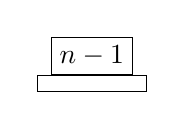
\begin{tikzpicture}
\node at (0,0) {\smallbrick};
\node at (0,-0.35) {\bigbrick};
\end{tikzpicture}}

\node[plate] (v4) at (1.9,3.9) {\smallbrick};
\node[gray,opacity=0.5] at  (v4) {$A$};
\node[plate] (v5) at (4.9,3.9) {\bigbrick};
\node[gray,opacity=0.5] at (v5) {$B$};
\node[plate] (v6) at (3.4,1.4) {};
\node[gray,opacity=0.5] at (v6) {$T$};

\draw[->,gray]  (v4) edge (v5);
\draw[->,red,line width=1pt]  (v5) edge node[right]{1} (v6);
\draw[->,gray]  (v6) edge (v4);

\end{tikzpicture}
